\documentclass[12pt]{article}
\usepackage[a4paper, total={6in, 9in}]{geometry}
\usepackage{graphicx}
\graphicspath{ {./images/output/} }
\usepackage{caption}
\usepackage[english]{babel}
\usepackage{titling}
\usepackage{float}
\usepackage{amsmath}
\usepackage{minted}
\usepackage{multicol}
% \usepackage{array}
% \usepackage{setspace}
% \usepackage{placeins}
\usepackage{parskip}

% \usepackage{lipsum}

\title{Design and Observe the Characteristics Curve of CMOS Circuit}
\author{}
\date{}

\pagenumbering{gobble}
\begin{document}
\vspace*{\fill}
\begin{center}

    \emph{Heaven's Light is Our Guide} \\
    \textbf{Rajshahi University of Engineering and Technology} \\

    \begin{figure}[H]
        \centering
        
\includegraphics[scale=.34]{images/RUET_logo.png}
        \label{fig:ruet_logo}
    \end{figure}
    \vspace{5mm}

    \textbf{Course Code}\\
    ECE 4128\\
    \vspace{3mm}
    \textbf{Course Title}\\
    VLSI Design

    \vspace{5mm}
    \textbf{Experiment Date:} {July 4, 2025},\\
    \textbf{Submission Date:} {August 11, 2025}\\

    \vspace{5mm}
    \textbf{Lab Report 2: \\
        Implementation of NMOS Ratio-less Inverter.}

    \vspace{15mm}

    \begin{tabular}{c|c}
        \textbf{Submitted to} & \textbf{Submitted by} \\
        Moloy Kumar Ghosh     &                       \\
        Lecturer              &                       \\
        Dept of ECE, RUET     & Md. Tajim An Noor     \\
        \&                    & Roll: 2010025         \\
        Md. Faysal Ahamed     &                       \\
        Lecturer              &                       \\
        Dept of ECE, RUET     &                       \\
    \end{tabular}

\end{center}
\vspace*{\fill}


\pagebreak

\tableofcontents

\pagebreak
\pagenumbering{arabic}
\maketitle

\section*{Task}
\addcontentsline{toc}{section}{Task}
Design and observe the characteristics curve of CMOS circuits using the following equations:

\begin{enumerate}
  \item \textbf{Equation I:} \( Y = \overline{(A + B) \cdot C} \)
  \item \textbf{Equation II:} \( Y = A\overline{B} + ABC \)
\end{enumerate}

For each equation:
\begin{itemize}
  \item Design the corresponding CMOS logic gate schematic.
  \item Simulate the circuit to obtain the output characteristics curve.
  \item Analyze the output waveform and discuss the behavior of the circuit.
\end{itemize}

\section*{Theory}
\addcontentsline{toc}{section}{Theory}
Complex CMOS logic gates implement Boolean functions in a single stage, offering greater efficiency compared to constructing the same function from multiple NAND or NOR gates~\cite{WesteHarrisCMOS}. These gates are composed of a pull-up network (PUN) using PMOS transistors and a pull-down network (PDN) using NMOS transistors. The PDN provides a path to ground $(V_{SS})$ when the output should be logic '$0$', while the PUN connects the output to the supply voltage $(V_{DD})$ when the output should be logic '$1$'. The PUN is the logical dual of the PDN, meaning series connections in one correspond to parallel connections in the other~\cite{RabaeyDigitalIC}.

\textbf{Equation I:} \( Y = \overline{(A + B) \cdot C} \)
This equation describes a 2-1 AND-OR-Invert (AOI21) gate~\cite{WesteHarrisCMOS}.

\begin{itemize}
  \item The pull-down network implements the logic \((A+B)\cdot C\), which consists of two parallel NMOS transistors (for A and B) in series with a third NMOS transistor (for C)~\cite{RabaeyDigitalIC}.
  \item The complementary pull-up network implements \((\overline{A}\cdot \overline{B})+\overline{C}\), realized by two series PMOS transistors (for A and B) in parallel with a third PMOS transistor (for C)~\cite{WesteHarrisCMOS}.
\end{itemize}

\begin{multicols}{2}
  \begin{table}[H]
    \centering

    \begin{tabular}{|c|c|c|c|}
      \hline
      A & B & C & Y \\
      \hline
      0 & 0 & 0 & 1 \\
      0 & 0 & 1 & 1 \\
      0 & 1 & 0 & 1 \\
      0 & 1 & 1 & 0 \\
      1 & 0 & 0 & 1 \\
      1 & 0 & 1 & 0 \\
      1 & 1 & 0 & 1 \\
      1 & 1 & 1 & 0 \\
      \hline
    \end{tabular}
    \caption{Truth Table for \( Y = \overline{(A + B) \cdot C} \)}
  \end{table}

  \begin{figure}[H]
    \centering
    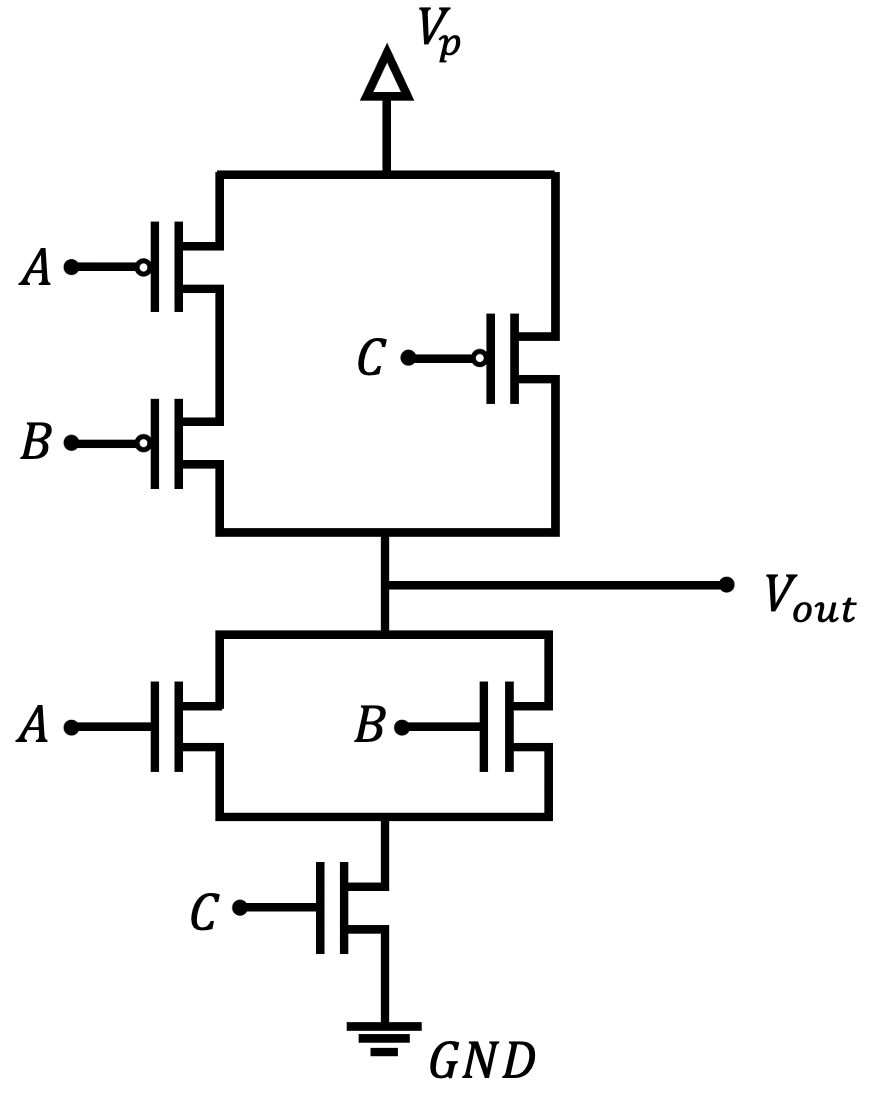
\includegraphics[width=.3\textwidth]{ck1.png}
    \caption{Connection diagram of the CMOS circuit for \( Y = \overline{(A + B) \cdot C} \)}
  \end{figure}
\end{multicols}

\textbf{Equation II:} \( Y = A\overline{B} + ABC \)

\begin{itemize}
  \item The pull-down network (PDN) implements the logic for (after simplification) \( \overline{A} + B\overline{C} \). This requires one NMOS transistor for \( \overline{A} \) (A input inverted), and a branch with NMOS transistors for \( B\overline{C} \) (B in series with C inverted), both branches connected in parallel~\cite{WesteHarrisCMOS,RabaeyDigitalIC}.
  \item The pull-up network (PUN) implements the dual logic, which for \( Y = A\overline{B} + ABC \) is \( A(\overline{B} + C) \). This is realized by two PMOS transistors for B and C in parallel, both in series with a PMOS transistor for A~\cite{WesteHarrisCMOS}.
  \item The circuit implements the function \( Y = \overline{A} + B\overline{C} \), which can be realized efficiently using CMOS logic~\cite{RabaeyDigitalIC}.
\end{itemize}

\begin{multicols}{2}
  \begin{table}[H]
    \centering
    \caption{Truth Table for \( Y = A\overline{B} + ABC \)}
    \begin{tabular}{|c|c|c|c|}
      \hline
      A & B & C & Y \\
      \hline
      0 & 0 & 0 & 0 \\
      0 & 0 & 1 & 0 \\
      0 & 1 & 0 & 0 \\
      0 & 1 & 1 & 0 \\
      1 & 0 & 0 & 1 \\
      1 & 0 & 1 & 1 \\
      1 & 1 & 0 & 0 \\
      1 & 1 & 1 & 1 \\
      \hline
    \end{tabular}
  \end{table}

  \begin{figure}[H]
    \centering
    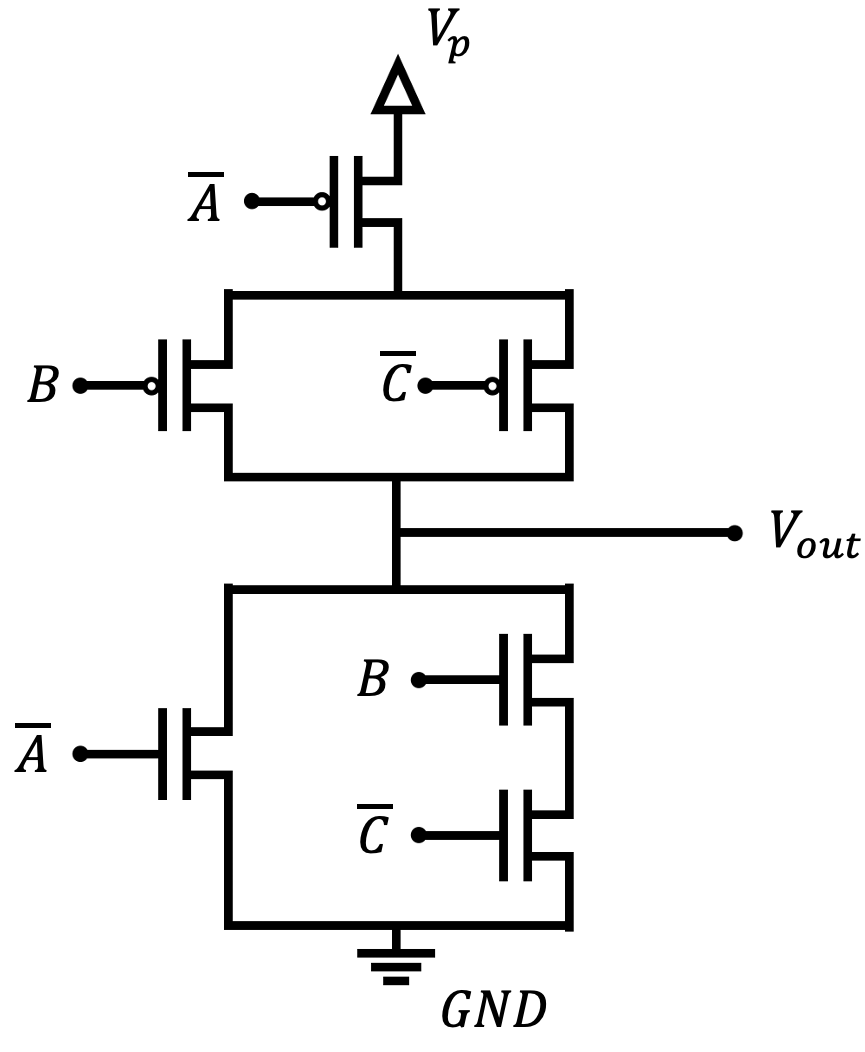
\includegraphics[width=.3\textwidth]{ck2.png}
    \caption{Connection diagram of the CMOS circuit for \( Y = A\overline{B} + ABC \)}
  \end{figure}
\end{multicols}

\section*{Used Tools}
\addcontentsline{toc}{section}{Used Tools}
\begin{itemize}
  \item Microwind
  \item MS Word
  \item MS PowerPoint
  \item \LaTeX
\end{itemize}

\section*{Circuit Schematic in Microwind}
\addcontentsline{toc}{section}{Circuit Schematic in Microwind}

\begin{figure}[H]
  \centering
  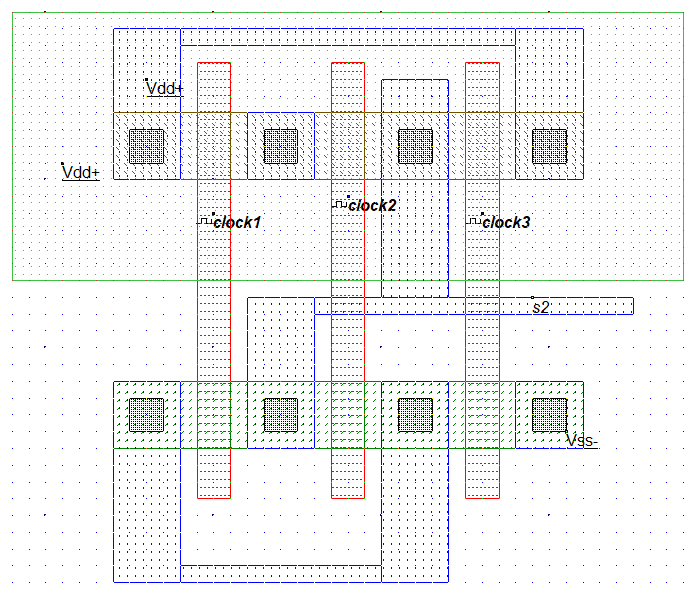
\includegraphics[width=.9\textwidth]{ckt1.png}
  \caption{Connection diagram of the CMOS circuit for \( Y = \overline{(A + B) \cdot C} \)}
\end{figure}

\begin{figure}[H]
  \centering
  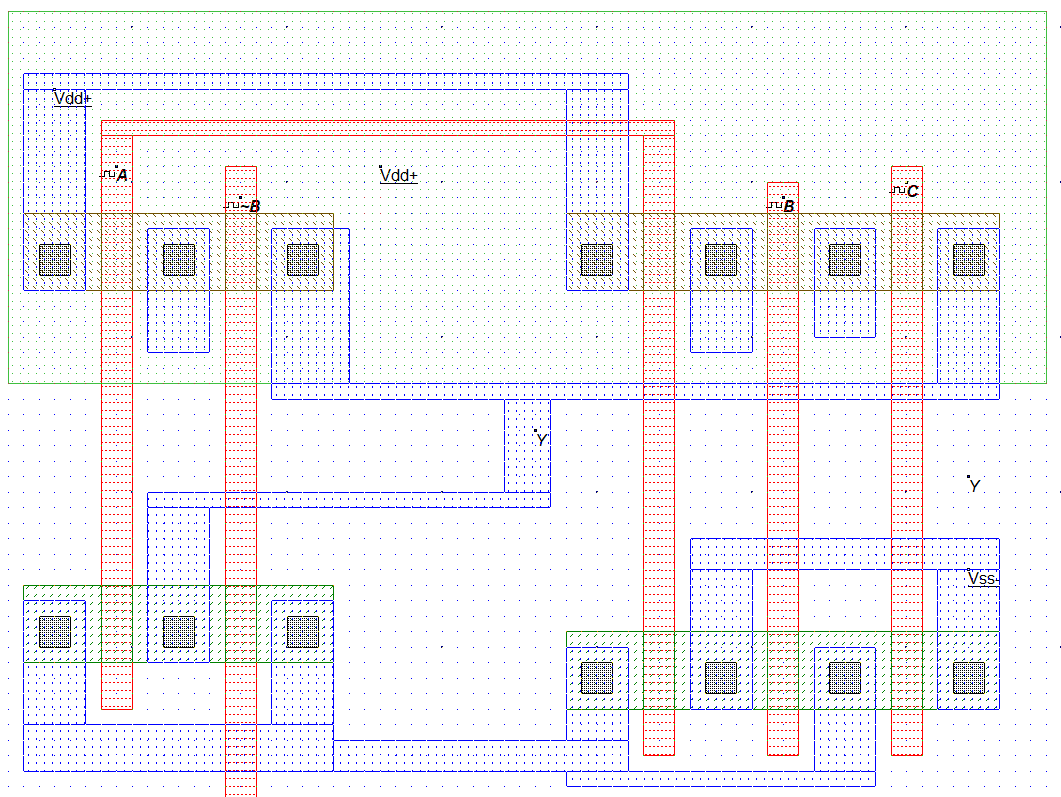
\includegraphics[width=.9\textwidth]{ckt2.png}
  \caption{Connection diagram of the CMOS circuit for \( Y = A\overline{B} + ABC \)}
\end{figure}

\section*{Output}
\addcontentsline{toc}{section}{Output}

\begin{figure}[H]
  \centering
  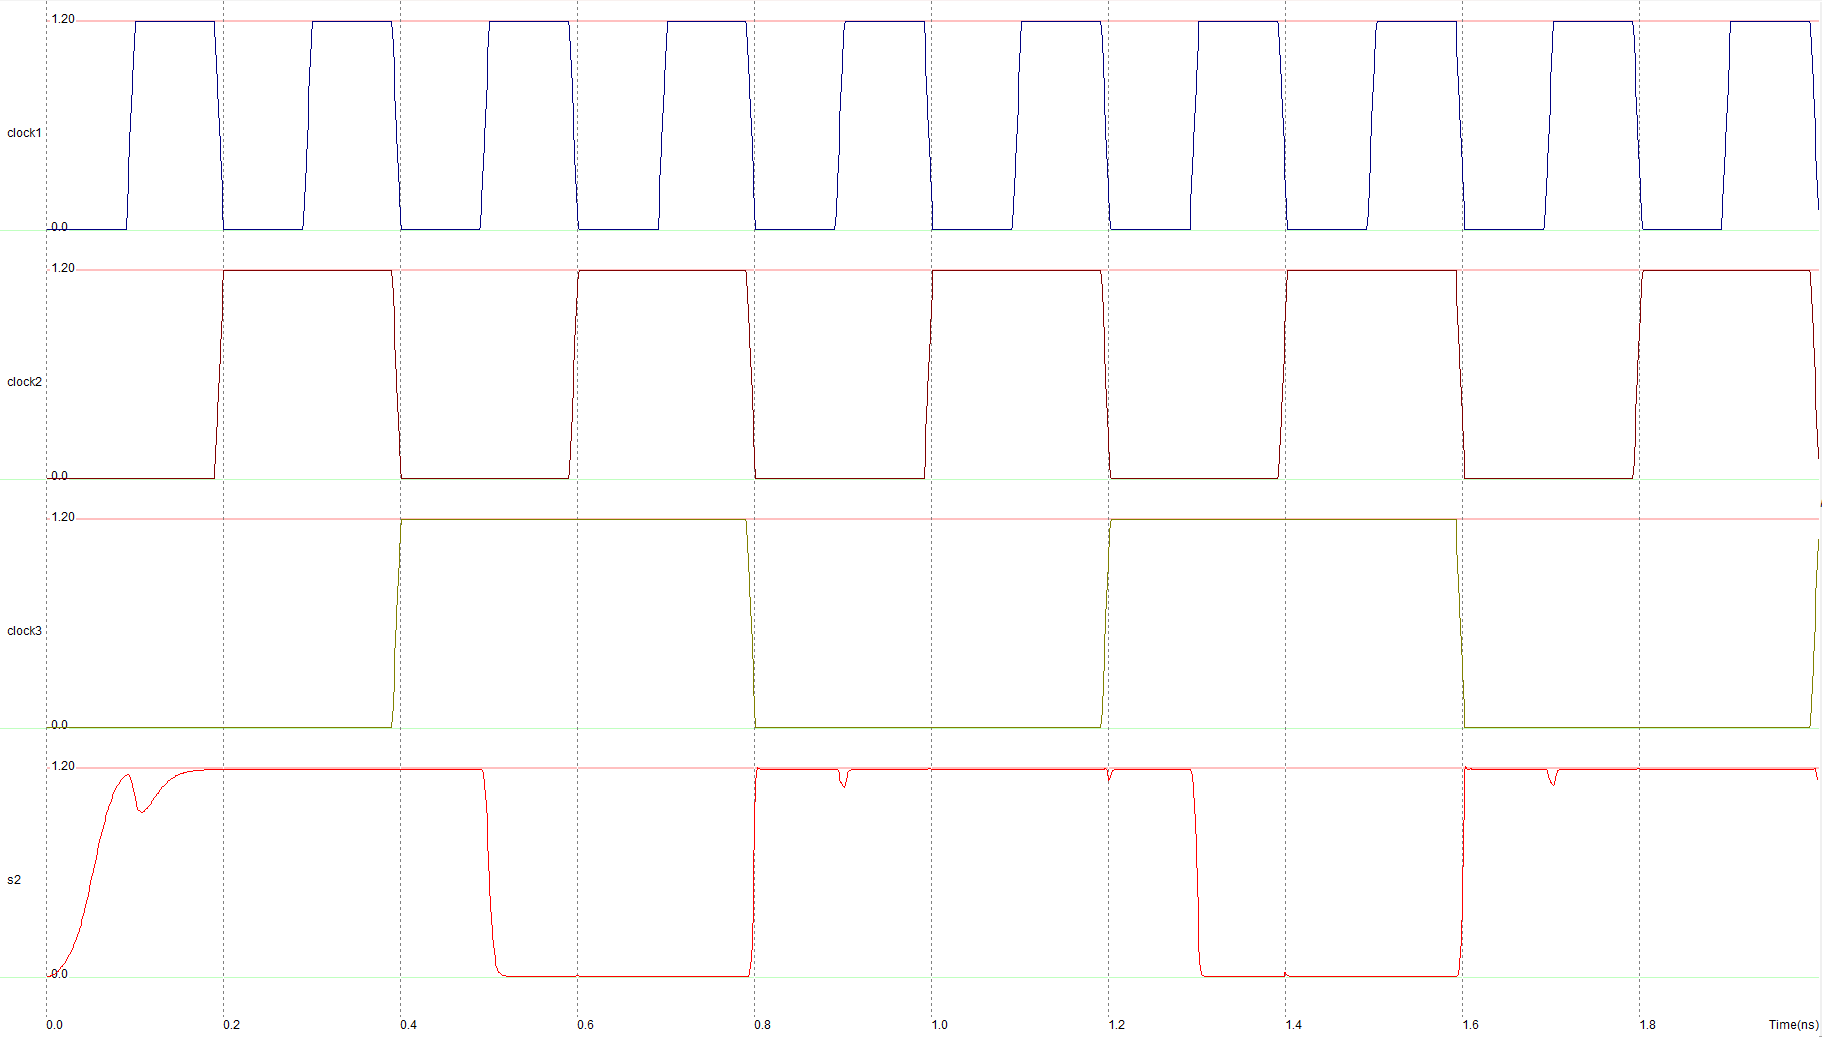
\includegraphics[width=.9\textwidth]{output1.png}
  \caption{Output Waveform of \( Y = \overline{(A + B) \cdot C} \)}
\end{figure}

\begin{figure}[H]
  \centering
  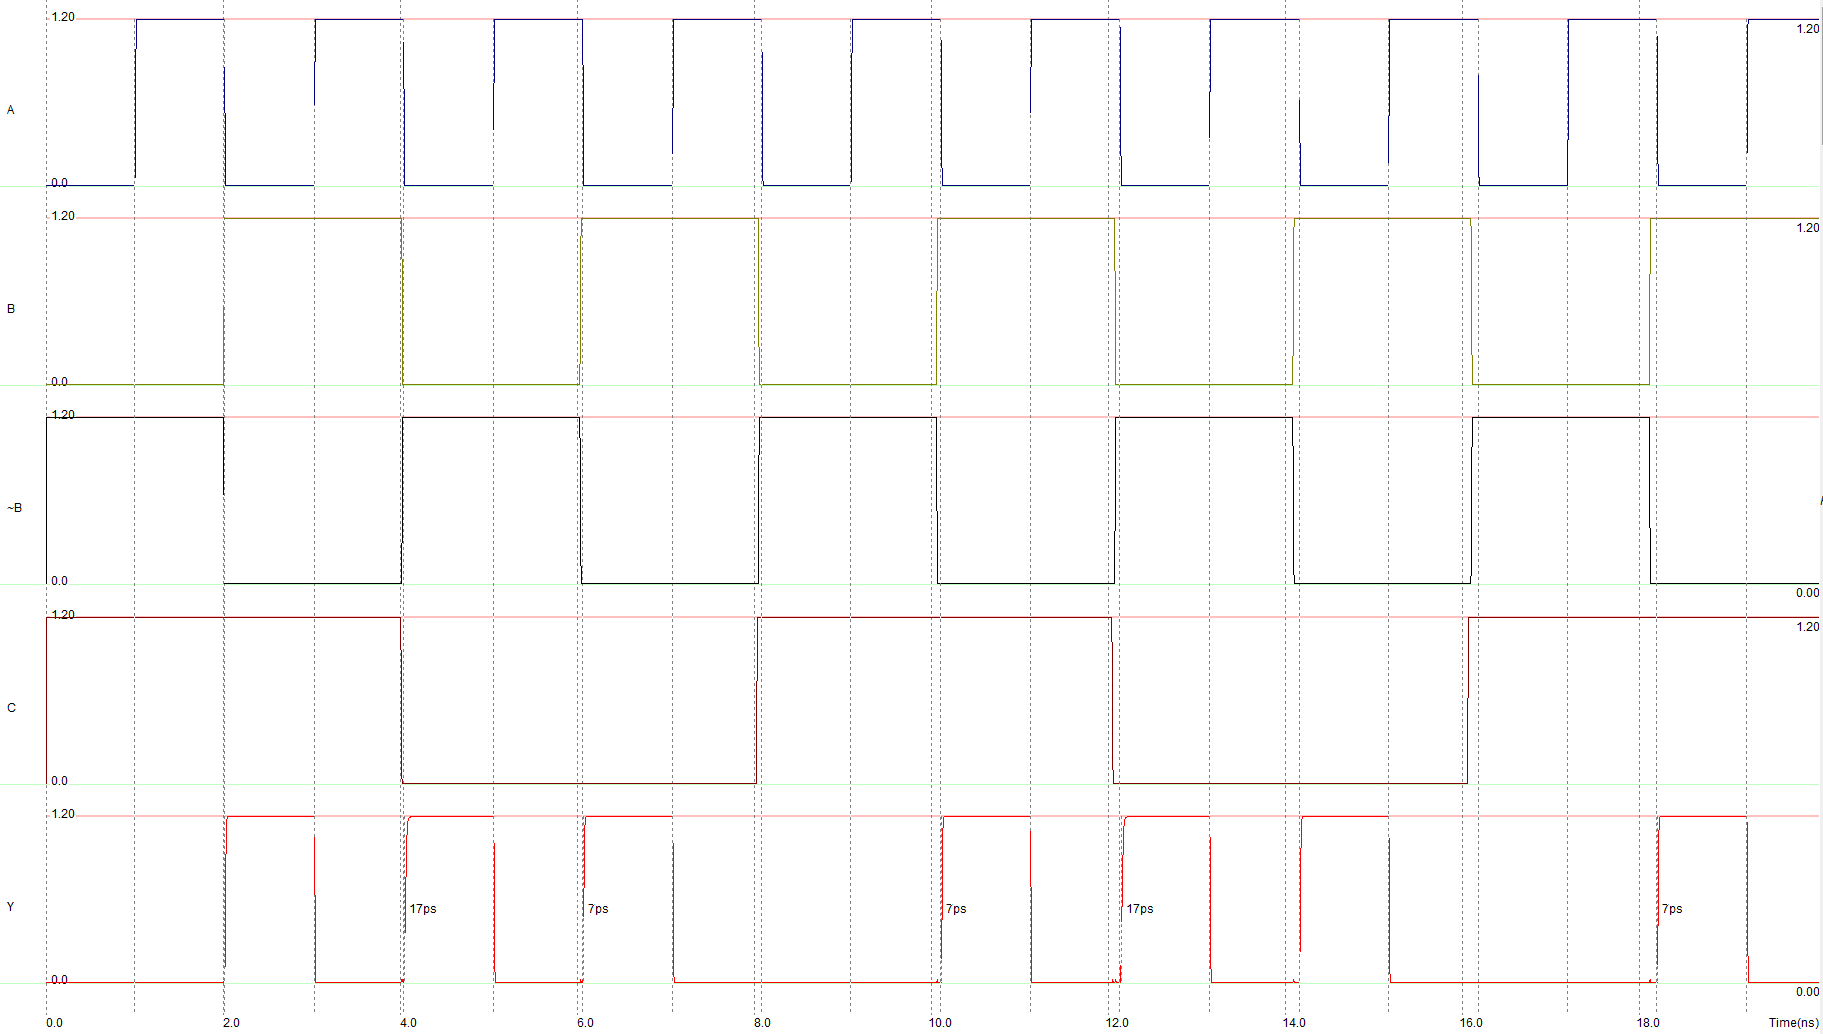
\includegraphics[width=.9\textwidth]{output2.png}
  \caption{Output Waveform of \( Y = A\overline{B} + ABC \)}
\end{figure}

\subsection*{Output Analysis}
\addcontentsline{toc}{subsection}{Output Analysis}
The complex CMOS circuits were implemented and simulated using Microwind. The resulting output waveforms align with the expected logical behavior as defined by the truth tables for each equation.

\textbf{Case I:} \( Y = \overline{(A + B) \cdot C} \)
\begin{itemize}
  \item When \( C = 0 \), the output remains HIGH (1) for all values of \( A \) and \( B \).
  \item When \( C = 1 \) and either \( A = 1 \) or \( B = 1 \), the output switches to LOW (0).
  \item When \( C = 1 \) and both \( A = 0 \) and \( B = 0 \), the output is HIGH (1).
  \item Simulation results confirm that the output is LOW only for input combinations (A,B,C) of (0,1,1), (1,0,1), and (1,1,1), consistent with the truth table.
\end{itemize}

\textbf{Case II:} \( Y = A\overline{B} + ABC \)
\begin{itemize}
  \item When \( A = 1 \) and \( B = 0 \), the output is HIGH (1), regardless of \( C \).
  \item When \( A = 1 \), \( B = 1 \), and \( C = 1 \), the output is HIGH (1).
  \item For all other input combinations, the output remains LOW (0).
  \item The simulation confirms that the output is HIGH only for (A,B,C) values of (1,0,0), (1,0,1), and (1,1,1), matching the truth table.
\end{itemize}

\section*{Discussion}
\addcontentsline{toc}{section}{Discussion}
This experiment explored the design and simulation of complex CMOS logic gates at the transistor level. By creating complementary pull-up (PMOS) and pull-down (NMOS) networks, complex Boolean functions such as AOI and OAI can be implemented in a single logic stage. This method is typically more efficient and faster than building the same function from multiple universal gates like NAND or NOR. The simulated output waveforms in Microwind closely matched the expected results from the truth tables, confirming both the dynamic and static behavior of the circuits.

\section*{Conclusion}
\addcontentsline{toc}{section}{Conclusion}
To summarize, the experiment confirmed the correct operation of complex CMOS circuits for the specified Boolean equations using Microwind. The observed results validated the design approach of using complementary pull-up and pull-down networks. This reinforces that complex logic functions can be directly and efficiently realized in CMOS technology, which is essential for integrated circuit design.


\bibliographystyle{IEEEtran}
\renewcommand{\bibname}{References}
\addcontentsline{toc}{section}{References}
\bibliography{ref}

\end{document}
